
\documentclass[a4paper,12pt]{article}

% Kodowanie i język
\usepackage[utf8]{inputenc}
\usepackage[T1]{fontenc}
\usepackage{babel}

% Matematyka
\usepackage{amsmath}
\usepackage{amssymb}

% Grafika
\usepackage{graphicx}
\usepackage{float}

% Wykresy i podpisy
\usepackage{caption}
\usepackage{subcaption}

% Tabele
\usepackage{booktabs}

% Marginesy
\usepackage[a4paper, margin=2.5cm]{geometry}
\usepackage{float}
% Linki
\usepackage{hyperref}

% Kod źródłowy
\usepackage{listings}
\usepackage{xcolor}

\lstset{
	basicstyle=\ttfamily\small,
	keywordstyle=\color{blue},
	commentstyle=\color{gray},
	stringstyle=\color{green!50!black},
	breaklines=true,
	frame=single
}

\title{Analiza częstotliwościowa sygnałów audio}
\author{Twoje imię i nazwisko}
\date{\today}


\begin{document}
	\begin{titlepage}
		\centering
		\vspace*{2cm}
		
		{\LARGE\bfseries Analiza i Przetwarzanie Dzwi\k{e}ku}\\[0.4cm]
		{\large Rok akademicki 2025/26}
		
		\vspace{2cm}
		
		{\Huge\bfseries Projekt 2}\\[0.6cm]
		{\Large Analiza częstotliwościowa}
		
		\vspace{3cm}
		
		{\Large
			Ryszard Czarnecki\\[0.3cm]
			J\'ozef Dubois
		}
		
		\vfill
		{\large Kwiecie\'n 2026}
	\end{titlepage}
	
	% --- Spis tresci ---
	\tableofcontents
	\newpage
	
\section{Opis aplikacji}


Aplikacja została zaimplementowana w języku Python z wykorzystaniem biblioteki \texttt{Streamlit}, poszerzono implementację z projektu 1. 


\subsection{Struktura projektu}
\begin{itemize}
	\item \textbf{parameters.py} -- obliczanie parametrów sygnału w dziedzinie czasu i częstotliwości,
	\item \textbf{windows.py} -- implementacja funkcji okienkowych,
	\item \textbf{spectrum.py} -- analiza widmowa, FFT, spektrogram, cepstrum, formanty,
	\item \textbf{pitch.py} -- estymacja częstotliwości podstawowej (autokorelacja, AMDF),
	\item \textbf{parameters\_over\_clip.py} -- parametry globalne dla całego sygnału,
	\item \textbf{main\_app.py} -- interfejs użytkownika oraz integracja wszystkich funkcji,
	\item \textbf{voiced\_unvoiced.py} -- wykrywanie fragmentów dźwięcznych/bezdźwięcznych,
	\item \textbf{silence\_detection.py} -- wykrywanie ciszy,
	\item \textbf{wav\_reader.py} -- wczytywanie ścieżek dźwiękowych.
\end{itemize}

\subsection{U\.zyte biblioteki}

\begin{itemize}
	\item \textbf{NumPy} -- operacje na tablicach numerycznych,
	normalizacja pr\'obek, fft,
	\item \textbf{Matplotlib} -- generowanie wykres\'ow (przebieg
	czasowy, parametry, pitch, klasyfikacja),
	\item \textbf{Streamlit} -- interfejs webowy z~widgetami (suwaki,
	pola numeryczne, przyciski pobierania),
	\item \textbf{Pandas} -- eksport parametr\'ow do pliku CSV.
\end{itemize}

\section{Opis metod}
Poniżej opisane są jedynie rzeczy dodane do aplikacji w ramach  projektu 2. Opis pozostałych metod znajduje się w sprawozdaniu raportu 1.

\subsection{Segmentacja sygnału}

Sygnał wejściowy dzielony jest na ramki o zadanej długości (w milisekundach) z określonym nakładaniem (overlap). Dla każdej ramki obliczane są parametry czasowe i częstotliwościowe.

Długość ramki wyrażona w próbkach:
\[
N = f_s \cdot \frac{T_{frame}}{1000}
\]

Przesunięcie między ramkami:
\[
hop = N \cdot (1 - overlap)
\]

\subsection{Transformata Fouriera (FFT)}

Do analizy widmowej wykorzystano szybką transformatę Fouriera (FFT) z biblioteki NumPy.

Widmo amplitudowe wyznaczane jest jako:
\[
X(k) = \left| \sum_{n=0}^{N-1} x(n) e^{-j 2\pi kn/N} \right|
\]

W implementacji wykorzystano tylko połowę widma (do częstotliwości Nyquista), co wynika z symetrii dla sygnałów rzeczywistych.

Dodatkowo obliczana jest skala logarytmiczna:
\[
X_{dB}(k) = 20 \log_{10}(X(k) + \epsilon)
\]

\subsection{Funkcje okienkowe}

Przed wykonaniem FFT sygnał jest mnożony przez funkcję okienkową w celu redukcji zjawiska przecieku widma (spectral leakage).

Zaimplementowano następujące okna:

\begin{itemize}
	\item okno prostokątne:
	\[
	w(n) = 1
	\]
	
	\item okno trójkątne:
	\[
	w(n) = 1 - \left| \frac{n - (N-1)/2}{(N-1)/2} \right|
	\]
	
	\item okno Hamminga:
	\[
	w(n) = 0.54 - 0.46 \cos\left(\frac{2\pi n}{N-1}\right)
	\]
	
	\item okno Hann (von Hanna):
	\[
	w(n) = 0.5 \left(1 - \cos\left(\frac{2\pi n}{N-1}\right)\right)
	\]
	
	\item okno Blackmana:
	\[
	w(n) = 0.42 - 0.5 \cos\left(\frac{2\pi n}{N-1}\right) + 0.08 \cos\left(\frac{4\pi n}{N-1}\right)
	\]
	
\end{itemize}

Dla każdej funkcji analizowany jest zarówno przebieg w dziedzinie czasu, jak i jej widmo.

\subsection{Widmo dla całego sygnału i pojedynczej ramki}

Aplikacja umożliwia:

\begin{itemize}
	\item analizę FFT dla całego sygnału,
	\item analizę FFT dla wybranej ramki sygnału,
	\item porównanie wpływu różnych funkcji okienkowych na widmo.
\end{itemize}

Dla pojedynczej ramki prezentowane są:
\begin{itemize}
	\item sygnał oryginalny,
	\item sygnał po zastosowaniu okna,
	\item widmo amplitudowe,
	\item widmo w skali dB.
\end{itemize}

\subsection{Spektrogram}

Spektrogram został zaimplementowany samodzielnie poprzez:

\begin{enumerate}
	\item podział sygnału na ramki,
	\item zastosowanie funkcji okna,
	\item obliczenie FFT dla każdej ramki,
	\item zapisanie logarytmicznej amplitudy widma.
\end{enumerate}

Wynik przedstawiany jest jako mapa:
\begin{itemize}
	\item oś X -- czas,
	\item oś Y -- częstotliwość,
	\item kolor -- amplituda w dB.
\end{itemize}

Użytkownik może regulować:
\begin{itemize}
	\item długość ramki,
	\item overlap,
	\item funkcję okna.
\end{itemize}

\subsection{Cepstrum i estymacja częstotliwości podstawowej}

Cepstrum obliczane jest jako odwrotna transformata Fouriera logarytmu widma:

\[
c(n) = \mathcal{F}^{-1} \left( \log |\mathcal{F}(x(n))| \right)
\]

Na jego podstawie wyznaczana jest częstotliwość podstawowa $F_0$ poprzez znalezienie maksimum w odpowiednim zakresie quefrencji:

\[
F_0 = \frac{f_s}{q_{max}}
\]

gdzie $q_{max}$ to indeks maksimum cepstrum w zadanym zakresie.



Wynik prezentowany jest oddzielnie od autokorelacji i AMDF.

\subsection{Estymacja formantów}
Formanty wyznaczane są bezpośrednio z widma FFT poprzez wygładzenie obwiedni 
spektralnej ruchomą średnią i~detekcję lokalnych maksimów.

Wygładzanie realizowane jest jako splot widma amplitudowego z~oknem prostokątnym 
o~długości $k$:
\[
\tilde{X}(m) = \frac{1}{k} \sum_{i=m-k/2}^{m+k/2} X(i)
\]
Parametr $k$ dobierany jest tak, aby wygładzić harmoniczne sygnału mowy 
(rozłożone co $F_0 \approx 100$--$150$~Hz), zachowując jednocześnie szerokie 
rezonanse traktu głosowego (formanty).

Spośród wykrytych lokalnych maksimów wybierane są kandydaci spełniający warunek:
\[
f_{min} < f < f_{max}
\]
gdzie przyjęto $f_{min} = 90$~Hz oraz $f_{max} = 4000$~Hz. Zwracane jest 
$n$ najsilniejszych pików posortowanych według częstotliwości, interpretowanych 
jako kolejne formanty F1, F2, F3.

Należy zaznaczyć, że metoda ta jest przybliżona, w~przeciwieństwie do analizy 
LPC (Linear Predictive Coding), nie modeluje bezpośrednio charakterystyki traktu 
głosowego, przez co może identyfikować harmoniczne wysokiej energii zamiast 
rzeczywistych formantów. Stanowi jednak prostą i~poglądową metodę estymacji 
w~ramach analizy FFT.

\subsection{Interaktywność aplikacji}

Aplikacja umożliwia dynamiczną zmianę parametrów analizy:

\begin{itemize}
	\item długości ramki,
	\item overlap,
	\item zakresu $F_0$,
	\item wyboru funkcji okna,
	\item wyboru analizowanej ramki.
\end{itemize}

Dzięki temu możliwe jest obserwowanie wpływu parametrów na wyniki analizy w czasie rzeczywistym.

\section{Różnica między spółgłoskami a samogłoskami.}
Aby zbadać różnice między spółgłoskami a samogłoskami zbadano nagranie słowa ,,abe''. Zostało ono podzielone na trzy segmenty odpowiadające poszczególnym głoskom: samogłosce \textit{a}, spółgłosce \textit{b} oraz samogłosce \textit{e}. Dla każdego segmentu wyznaczono trzy pierwsze formanty (F1, F2, F3) na podstawie analizy cepstralnej i widmowej.

\subsection{Wyniki pomiarów}

\begin{table}[h]
	\centering
	\caption{Wartości formantów dla poszczególnych segmentów nagrania ,,abe'' policzonych dla widma FFT z oknem Prostokątnym.}
	\label{tab:formanty_abe}
	\begin{tabular}{|l|c|c|c|}
		\hline
		\textbf{Segment} & \textbf{F1 [Hz]} & \textbf{F2 [Hz]} & \textbf{F3 [Hz]} \\
		\hline
		a & 900{,}0 & 1025{,}0 & 1125{,}0 \\
		b & 277{,}7 & 333{,}3 & 355{,}6 \\
		e & 389{,}1 & 511{,}4 & 622{,}0 \\
		\hline
	\end{tabular}
\end{table}

\begin{figure}[H]
	\centering
	
	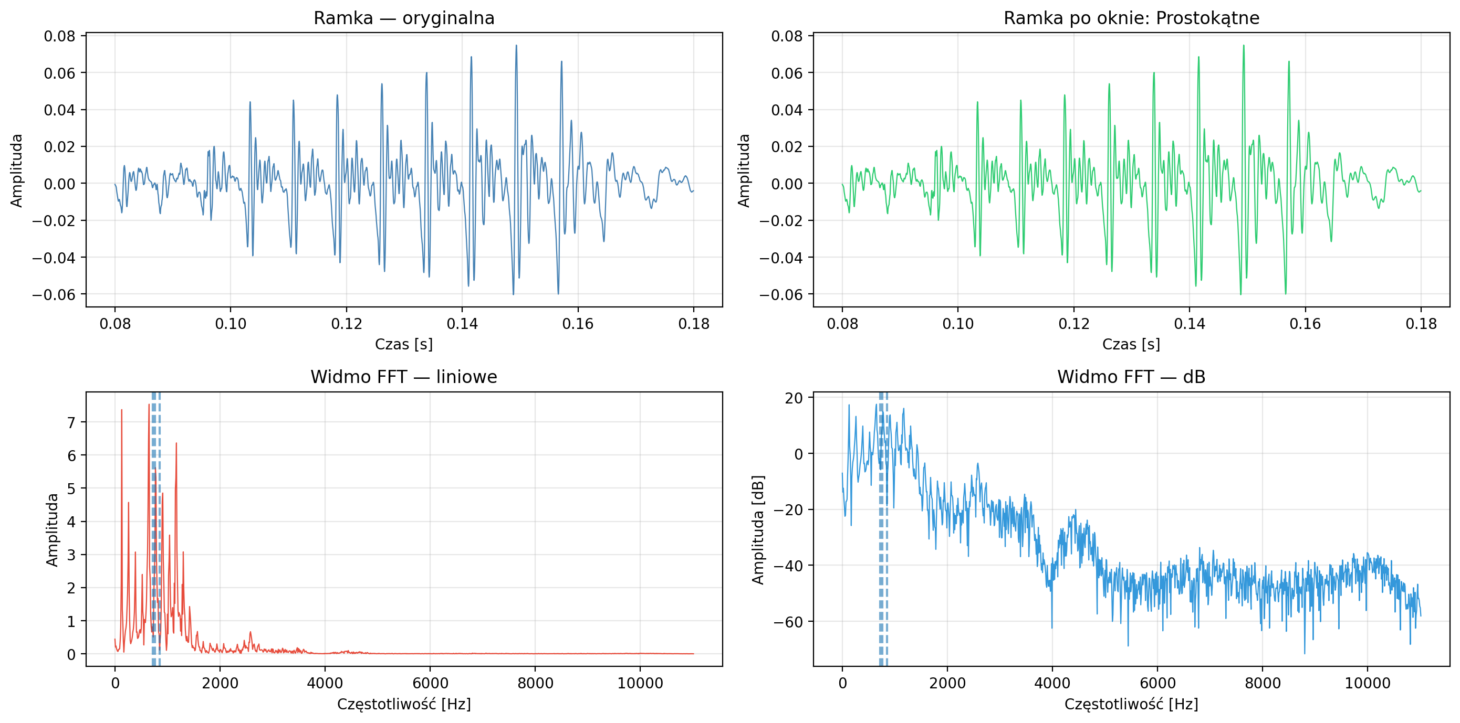
\includegraphics[width=0.8\textwidth]{abe_a_fft_formants}
	
	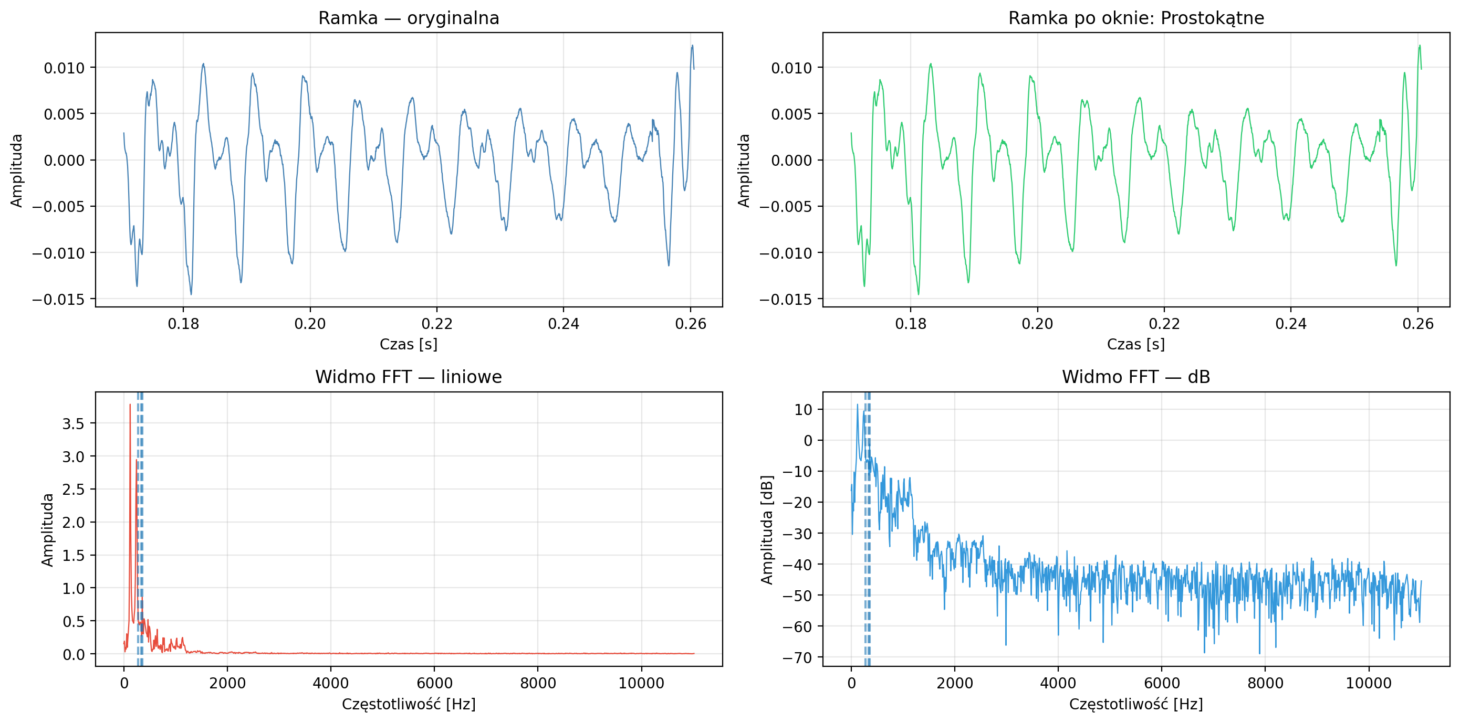
\includegraphics[width=0.8\textwidth]{abe_b_fft_formants}
	
	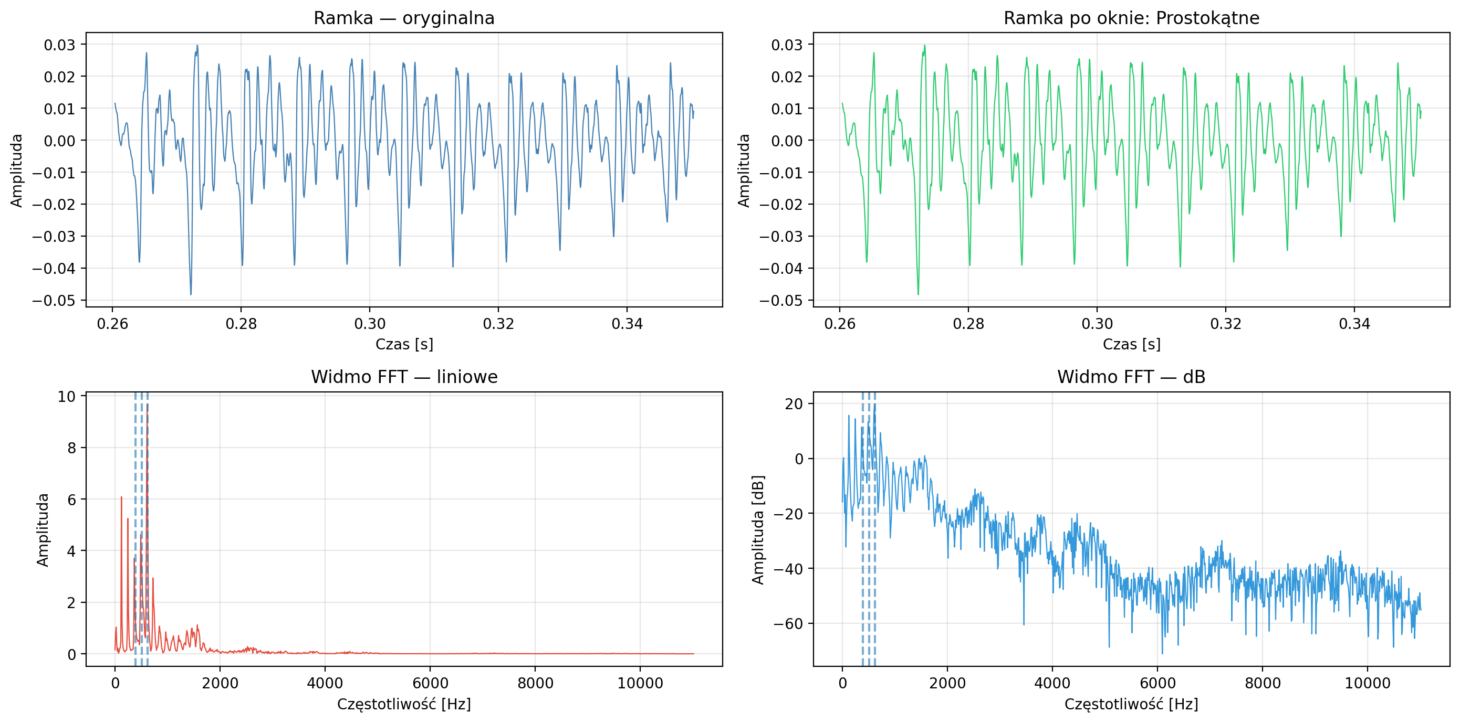
\includegraphics[width=0.8\textwidth]{abe_e_fft_formants}
	
	\caption{Widmo FFT z zaznaczonymi formantami dla segmentów \textit{a}, 
		\textit{b} oraz \textit{e}.}
	\label{fig:fft_formants}
\end{figure}

\subsection{Analiza wyników}
Uzyskane wartości formantów częściowo odbiegają od wartości referencyjnych podawanych 
w~literaturze fonetycznej. Dla samogłoski \textit{a} typowe wartości formantów 
(mężczyzna) wynoszą: F1~$\approx$~700--800~Hz, F2~$\approx$~1200--1400~Hz, 
F3~$\approx$~2500--2800~Hz. Dla samogłoski \textit{e}: F1~$\approx$~400--500~Hz, 
F2~$\approx$~1800--2200~Hz, F3~$\approx$~2500--2800~Hz.

Wartość F1 dla samogłoski \textit{a} (900~Hz) mieści się w~pobliżu przedziału 
referencyjnego, natomiast F2 i~F3 są wyraźnie zaniżone. Dla samogłoski \textit{e} 
F1 (389~Hz) jest zgodny z~literaturą, jednak F2 i~F3 są znacząco niższe od 
oczekiwanych. Rozbieżności te wynikają prawdopodobnie z~ograniczeń zastosowanej 
metody estymacji -- wygładzanie obwiedni spektralnej ruchomą średnią nie eliminuje 
w~pełni wpływu harmonicznych sygnału mowy, przez co algorytm może identyfikować 
harmoniczne wysokiej energii zamiast rzeczywistych formantów. Dokładniejszą estymację 
umożliwiłaby metoda LPC (Linear Predictive Coding), która modeluje obwiednię 
spektralną bez konieczności wygładzania.

Dla spółgłoski \textit{b} uzyskane wartości (F1~$\approx$~278~Hz, F2~$\approx$~333~Hz, 
F3~$\approx$~356~Hz) nie powinny być interpretowane jako formanty w~klasycznym sensie. 
Spółgłoska zwarta \textit{b} charakteryzuje się krótką okluzją, po której następuje gwałtowne uwolnienie energii. 
Na tak krótkim i~niekvazistacjonarnym fragmencie sygnału estymacja formantów metodą 
FFT jest z~założenia zawodna, a~uzyskane wartości odzwierciedlają raczej strukturę 
harmoniczną otaczających samogłosek lub artefakty numeryczne.


\subsubsection{Porównanie segmentów}


\begin{figure}[H]
	\centering
	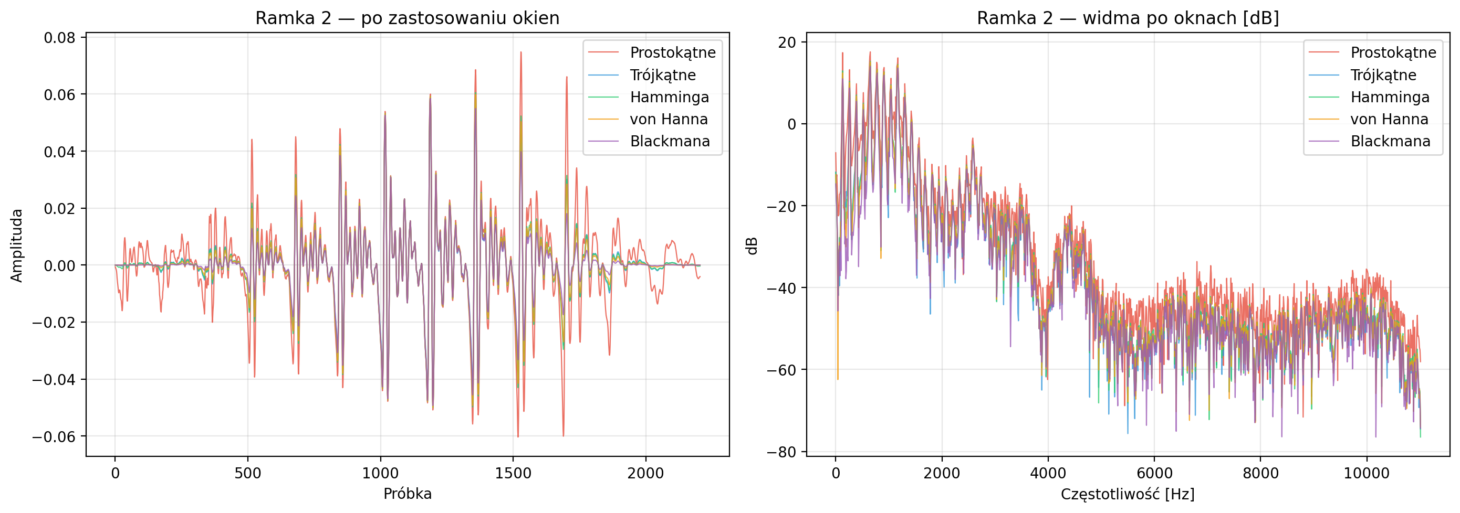
\includegraphics[width=0.85\textwidth]{abe_a_widma}\\[6pt]
	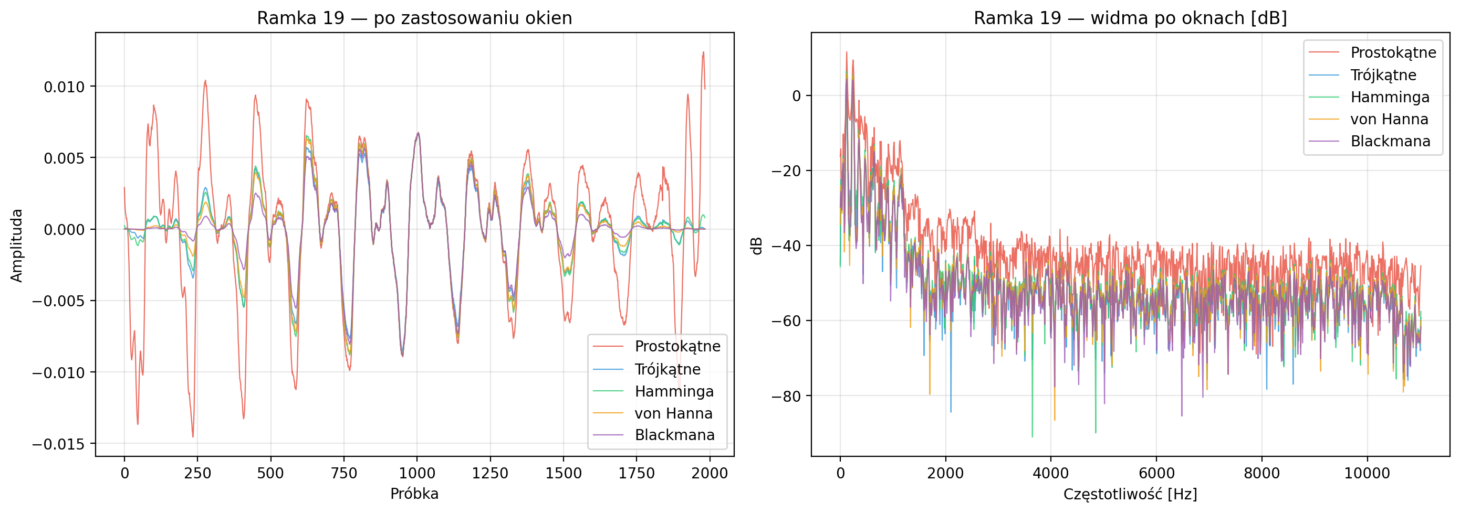
\includegraphics[width=0.85\textwidth]{abe_b_widma}\\[6pt]
	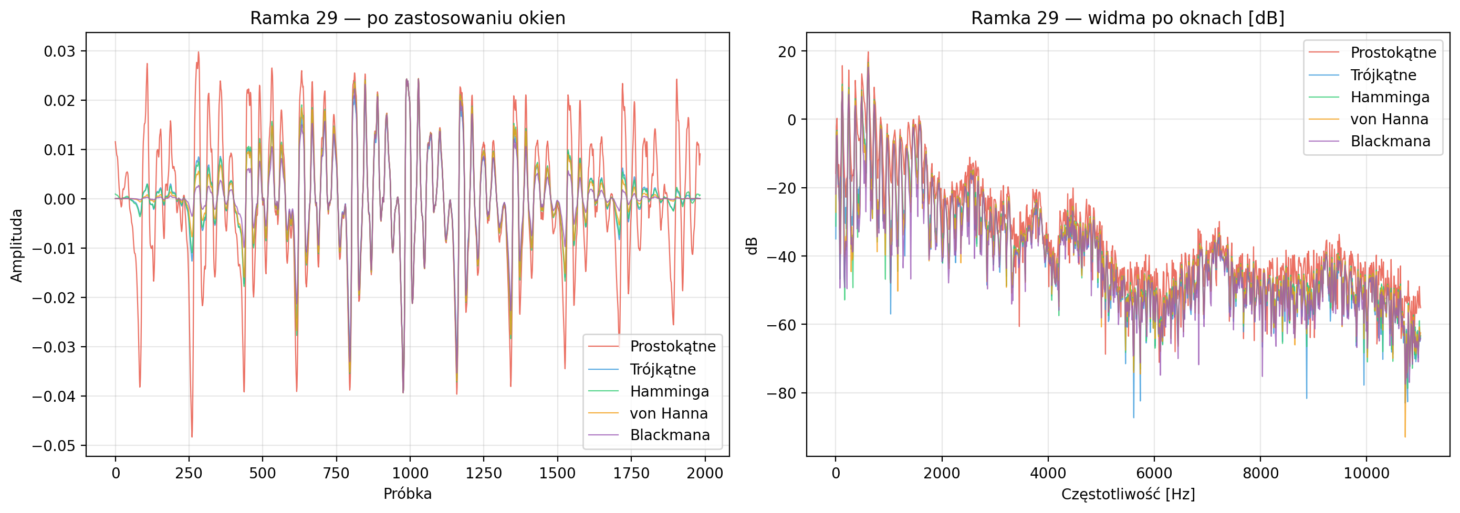
\includegraphics[width=0.85\textwidth]{abe_e_widma}
	\caption{Porównanie widm FFT dla różnych funkcji okna -- segmenty 
		\textit{a} (górny), \textit{b} (środkowy) i~\textit{e} (dolny).}
	\label{fig:widma_okna}
\end{figure}

Mimo że wartości bezwzględne nie odpowiadają typowym formantom, można zaobserwować 
pewne prawidłowości:
\begin{itemize}
	\item Segment \textit{a} wykazuje najwyższe wartości F1 i~F2 spośród wszystkich 
	segmentów (F1~=~900~Hz, F2~=~1025~Hz), co jest zgodne z~fonetyczną charakterystyką 
	samogłoski tylnej otwartej, szeroko otwarty trakt głosowy skutkuje wysokim F1.
	
	\item Segment \textit{e} ma niższe F1 (389~Hz) niż \textit{a}, co odpowiada 
	mniej otwartej artykulacji samogłoski przedniej. Różnica między F1 a~F2 jest 
	większa niż dla \textit{a}, co jakościowo odzwierciedla charakterystyczny 
	układ formantów samogłosek przednich.
	
	\item Dla segmentu \textit{b} uzyskane wartości (F1~=~278~Hz, F2~=~333~Hz, 
	F3~=~356~Hz) są najniższe i~skupione w~wąskim paśmie niskich częstotliwości. 
	Jak wspomniano wcześniej, nie należy ich interpretować jako formantów -- 
	mogą one odpowiadać składowym harmonicznym sąsiednich samogłosek lub artefaktom 
	wynikającym z~krótkości i~niekvazistacjonarności segmentu.
\end{itemize}

\subsubsection{Analiza spektrogramu i cepstrum}

\begin{figure}[H]
	\centering
	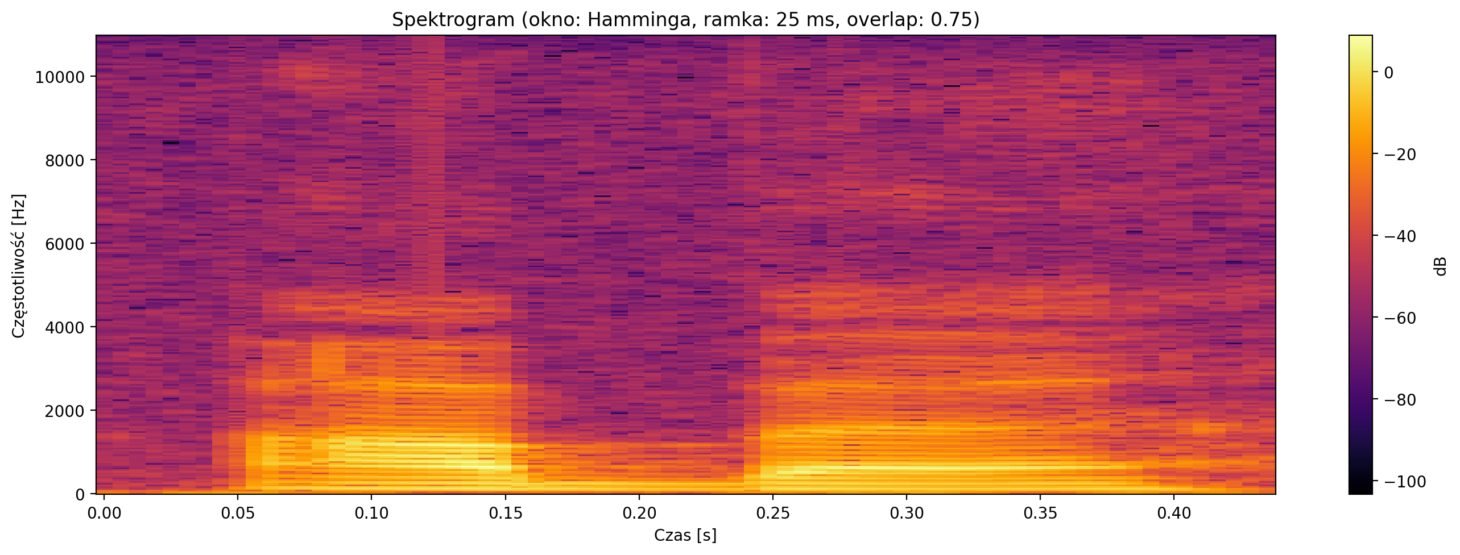
\includegraphics[width=0.85\textwidth]{abe_spektogram}
	\caption{Spektrogram nagrania ,,abe'' z widoczną strukturą harmoniczną 
		segmentów samogłoskowych.}
	\label{fig:spektrogram}
\end{figure}

\begin{figure}[H]
	\centering
	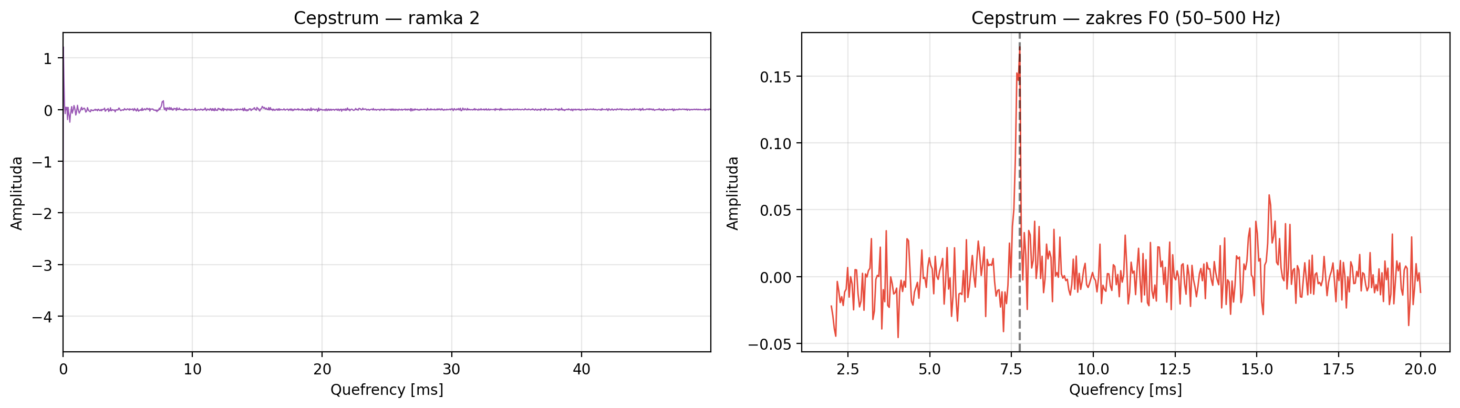
\includegraphics[width=0.85\textwidth]{abe_a_cepstum}\\[6pt]
	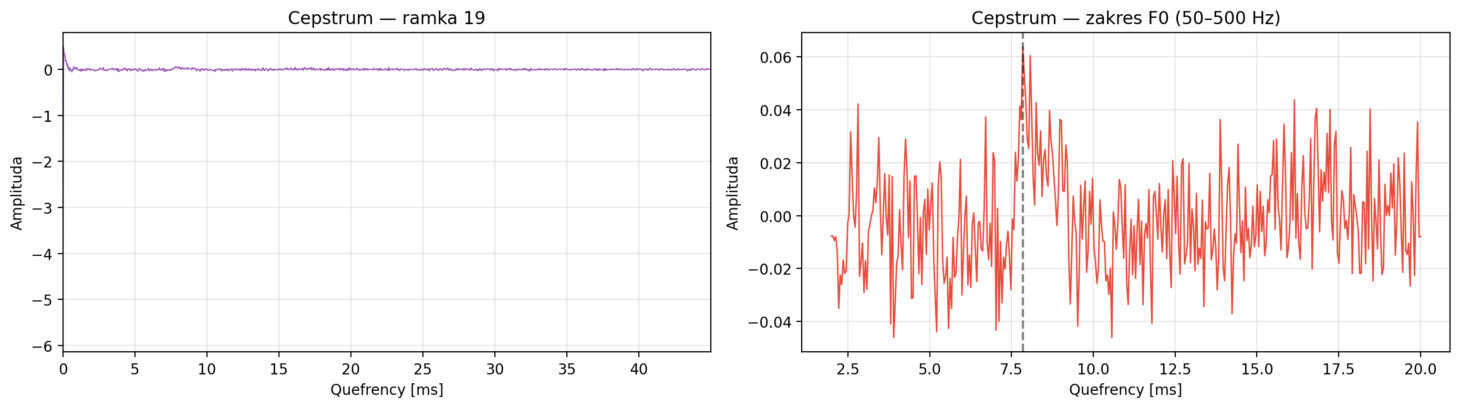
\includegraphics[width=0.85\textwidth]{abe_b_cepstum}\\[6pt]
	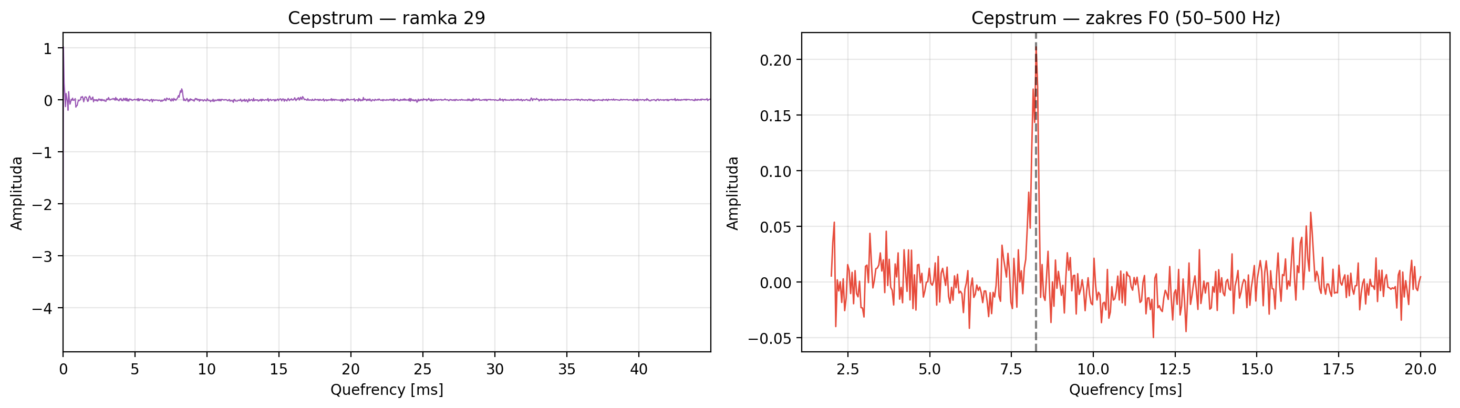
\includegraphics[width=0.85\textwidth]{abe_e_cepstum}
	\caption{Cepstrum segmentów \textit{a} (górny), \textit{b} (środkowy) 
		i~\textit{e} (dolny) z widocznym pikiem przy $\tau \approx 8$~ms 
		odpowiadającym F0~$\approx$~125~Hz.}
	\label{fig:cepstra}
\end{figure}



Spektrogram nagrania ,,abe'' uwidacznia wyraźne różnice między segmentami:

\begin{itemize}
	\item W~segmentach samogłoskowych (\textit{a}, \textit{e}) widoczna jest regularna struktura harmoniczna --- równomiernie rozłożone pasma energii odpowiadające kolejnym harmonicznym F0.
	\item Segment \textit{b} charakteryzuje się krótkim przerwaniem struktury harmonicznej (faza zwarcia) i~następującym szerokopasmowym impulsem (faza wybuchu).
	\item Analiza cepstralna wykazała wyraźny pik w~okolicach kwefrencji $\tau \approx 8$~ms, co odpowiada $F0 = 1/\tau \approx 125$~Hz. Pik ten jest dobrze widoczny w~segmentach dźwięcznych (\textit{a}, \textit{b}, \textit{e}).
\end{itemize}

\subsubsection{Wpływ funkcji okna}

Porównanie różnych funkcji okna (prostokątne, trójkątne, Hamminga, von Hanna, Blackmana) na widmo FFT wykazało:

\begin{itemize}
	\item Okno prostokątne daje najwęższe pasmo główne, ale największy poziom listków bocznych (spectral leakage), co utrudnia rozróżnienie bliskich składowych częstotliwościowych.
	\item Okna Hamminga i~von Hanna skutecznie tłumią listki boczne (o~ok.\ 40--50~dB) kosztem niewielkiego poszerzenia pasma głównego.
	\item Okno Blackmana zapewnia najlepsze tłumienie listków bocznych (ponad 70~dB), ale najszersze pasmo główne, co obniża rozdzielczość częstotliwościową.
\end{itemize}

\subsection{Wnioski}

\begin{enumerate}
	\item Wyznaczone wartości formantów nie odpowiadają wartościom referencyjnym z~literatury fonetycznej. Prawdopodobną przyczyną jest to, że algorytm identyfikuje piki harmonicznych F0 w~widmie zamiast rezonansów traktu głosowego (formantów). Poprawne wyznaczanie formantów wymaga zastosowania analizy LPC (Linear Predictive Coding) lub metody obwiedni widmowej.
	\item Pomimo tego ograniczenia, relacje między wartościami formantów poszczególnych segmentów zachowują pewną spójność z~oczekiwaniami fonetycznymi (np.\ wyższe wartości dla \textit{b} wynikające z~szerokopasmowego charakteru spółgłoski zwartej).
	\item Analiza cepstralna poprawnie identyfikuje częstotliwość podstawową F0~$\approx$~125~Hz, co jest wartością typową dla męskiego głosu.
	\item Porównanie funkcji okna potwierdza teoretyczny kompromis między rozdzielczością częstotliwościową a~tłumieniem listków bocznych. Dla analizy mowy okno Hamminga stanowi dobry kompromis.
	\item Spektrogram poprawnie wizualizuje strukturę czasowo-częstotliwościową nagrania, umożliwiając rozróżnienie segmentów samogłoskowych i~spółgłoskowych.
\end{enumerate}

\section{Podsumowanie}

W~ramach projektu zaimplementowano aplikację do analizy częstotliwościowej sygnałów 
dźwiękowych, stanowiącą rozbudowę projektu~1. Aplikacja umożliwia analizę widmową 
poprzez FFT dla całego sygnału oraz wybranych ramek, zastosowanie pięciu funkcji 
okienkowych, rysowanie spektrogramu z~regulowanymi parametrami, estymację 
częstotliwości podstawowej metodą cepstralną oraz wyznaczanie formantów.

Analiza nagrania słowa ,,abe'' pozwoliła zaobserwować wyraźne różnice między 
samogłoskami a~spółgłoską w~dziedzinie częstotliwości. Segmenty samogłoskowe 
(\textit{a}, \textit{e}) charakteryzują się regularną strukturą harmoniczną 
widoczną zarówno w~widmie FFT, jak i~na spektrogramie. Segment spółgłoski zwartej 
\textit{b} wyróżnia się krótką przerwą w~strukturze harmonicznej (faza okluzji) 
i~szerokopasmowym impulsem wybuchu -- cechy te są wyraźnie rozróżnialne na 
spektrogramie.

Analiza cepstralna poprawnie wyznaczyła częstotliwość podstawową $F_0 \approx 125$~Hz, 
co odpowiada typowej wartości dla głosu męskiego. Estymacja formantów metodą 
wygładzania obwiedni spektralnej dała wyniki częściowo zgodne z~oczekiwaniami 
fonetycznymi, F1 samogłosek mieści się w~pobliżu wartości referencyjnych, 
natomiast F2 i~F3 są zaniżone ze względu na ograniczenia metody. Dokładniejszą 
estymację umożliwiłoby zastosowanie analizy LPC.

Porównanie funkcji okienkowych potwierdziło teoretyczny kompromis między 
rozdzielczością częstotliwościową a~tłumieniem listków bocznych. Okno prostokątne 
zapewnia najlepszą rozdzielczość kosztem wycieku widma, natomiast okno Blackmana 
minimalizuje wyciek kosztem rozdzielczości. Dla analizy sygnału mowy okno Hamminga 
stanowi dobry kompromis między obiema właściwościami.

\end{document}